\newcommand{\figTimingArbitration}{%
  \centering
  \footnotesize
  \begin{tikztimingtable}[timing/wscale=6.0,timing/slope=.3]
    %          IrrrrrrRLLL A dddddddddD L ttttttttT 0
    CLK In   & H      HHHC C          C C         C C\\
    CLK Out  & H      HHHC C          C C         C C\\
    Data In  & H      HHHH H .2H.2L.6H  H .4H.6L    L\\
    Data Out & H.5H.5L LLL L L          L .4H.6L    L\\
             & \\
    \\
    CLK In   & H      HHHC C           CC         C C\\
    CLK Out  & H      HHHC C           CC         C C\\
    Data In  & H.7H.3L LLL L L          L .4L.2H.4L L\\
    Data Out & H.7H.3L LLL L L          L .4L.2H.4L L\\
             & \\
    \\
    CLK In   & H      HHHC C           CC         C C\\
    CLK Out  & H      HHHC C           CC         C C\\
    Data In  & H.8H.2L LLL L L          L .6L.2H.2L L\\
    Data Out & H      LLLL L H          H L         L\\
             & \\
    \\
    CLK In   & H      HHHC C           CC         C C\\
    CLK Out  & H      HHHC C           CC         C C\\
    Data In  & H.2H.8L LLL L .2L.8 H    H .2H.8L    L\\
    Data Out & H      HHHH H .2L.8 H    H .2H.8L    L\\
    Int Clk  & X      XXCC C           CC         C C\\
             & \\
  \extracode
    \begin{pgfonlayer}{background}
      \begin{scope}[semithick,dashed]
        \vertlines[color=gray]{6,30,36,...,\twidth}
        \vertlines[color=red]{36,48,...,\twidth}
      \end{scope}
    \end{pgfonlayer}

    \begin{scope}
      [font=\bf\sffamily,shift={(-5.5em,-1.5)},anchor=east,color=blue]
      \node [rotate=45] at (  0,   0) {1};
      \node [rotate=45] at (  0, -12) {2};
      \node [rotate=45] at (  0, -24) {3};
      \node [rotate=45] at (  0, -36) {Ctl};
    \end{scope}

    \begin{scope}
      [font=\sc\scriptsize,shift={(-1,5.5)},anchor=north,align=center]
      \node [rotate=45] at (30, 0) {Arbi-\\tration};
      \node [rotate=45] at (36, 0) {Prio\\Drive};
      \node [rotate=45] at (42, 0) {Prio\\Latch};
      \node [rotate=45] at (48, 0) {Drive\\Bit~0};
      \node [rotate=45] at (54, 0) {Latch\\Bit~0};
      \node [rotate=45] at (60, 0) {Drive\\Bit~1\ldots};
    \end{scope}

    \begin{scope}
      [font=\scriptsize]
      \draw[orange,thick]  (30,  -5) ellipse (1.25 and 2.5);
      \draw[orange,thick]  (30, -29) ellipse (1.25 and 2.5);
      \draw(26.5,-8.5)  node[align=center] {Won\\Arbitration};
      \draw(26.5,-32.5) node[align=center] {Lost\\Arbitration};

      \draw[cyan,thick]    (36,  -5) ellipse (1.25 and 2.5);
      \draw(36, -9) node[align=center,fill=white,fill opacity=.75] {Does Not\\Forward};

      \draw[olive,thick]   (42,  -5) ellipse (1.25 and 2.5);
      \draw[olive,thick]   (42, -29) ellipse (1.25 and 2.5);
      \draw(45,-8.5)  node[align=center] {Prio Req\\Back Off};
      \draw(45,-32.5) node[align=center] {Won Prio\\Arbitration};
    \end{scope}

    \begin{scope}
      [color=blue]
      \draw
        (7.2,-39) node[] (TL) {}
        (7.2,-50) node[] (BL) {}
        ( 24,-36) node[] (TR) {}
        ( 24,-50) node[] (BR) {};
      \node[right=6 of BL] (tlong) {$t_{long}$};
      \draw[<-] (BL.east) -- (tlong.west);
      \draw[->] (tlong.east) -- (BR.west);
      \draw[dashed] (TL) -- (BL);
      \draw[dashed] (TR) -- (BR);
    \end{scope}

    \draw (6, -46.5) -- +(0,-.2)
      node [below,inner sep=2pt] {\scalebox{.75}{\footnotesize0}};
    \foreach \n [evaluate=\n as \l using int((\n-24)/6)] in {30,36,...,\twidth}
      \draw (\n,-46.5) -- +(0,-.2)
        node [below,inner sep=2pt] {\scalebox{.75}{\footnotesize\l}};
  \end{tikztimingtable}
  \caption{
    \bus Arbitration. To begin a transaction, nodes pull down on data.
    Here we show node~1 and node~3 requesting the bus at nearly the same time
    (node~1 shortly after node~3). Node~1 initially wins arbitration, but
    node~3 uses the priority arbitration cycle to claim the bus. The
    propogation delay of the data line between nodes is exaggurated to show
    the shoot-through nature of \bus.
  }
  \label{fig:arbitration}
} % End \figTimingArbitration


\newcommand{\figTimingInterrupt}{%
\hspace{-1em}
\noindent\makebox[\textwidth]{%
  \footnotesize
  \begin{tikztimingtable}[timing/wscale=3.0,timing/slope=.3]
    %          10011 EE EE IIIIII SS X110 0II
    CLK In   & CCCCC CC CC CHHHHH HC CCCC CCC\\
    CLK Out  & CCCCC CC CC CHHHHH HC CCCC CCC\\
    Data In  & HHLLH HH HH HCCCCC CH HHHL LHH\\
    Data Out & HHLLH HH HH HCCCCC CH HHHL LHH\\
             & {1D{Data 1}}{2D{Data 0}}{2D{Data 1}}
               {2D{Data 1}}{2D{Data 1}}{6D{Interrupt}}{2D{Switch Role}}
               {2D{Ctl Bit 0}}{2D{ACK=True}}{2D{Idle}}{1D{\ldots}} \\
    \\
    % TX Node
    CLK In   & CCCCC CC CC CHHHHH HC CCCC CCC\\
    CLK Out  & CCCCC CH HH HHHHHH HH CCCC CCC\\
    Data In  & HHLLH HH HH HCCCCC CH HHHL LHH\\
    Data Out & HHLLH HH HH HCCCCC CH HHHL LHH\\
             & {1D{Data 1}}{2D{Data 0}}{2D{Data 1}}
               {4D{Req Interrupt}}{6D{Interrupt}}{2D{Switch Role}}
               {2D{EoM=True}}{2D{Ctl Bit 1}}{2D{Idle}}{1D{\ldots}} \\
    \\
    CLK In   & CCCCC CH HH HHHHHH HH CCCC CCC\\
    CLK Out  & CCCCC CH HH HHHHHH HH CCCC CCC\\
    Data In  & HHLLH HH HH HCCCCC CH HHHL LHH\\
    Data Out & HHLLH HH HH HCCCCC CH HHHL LHH\\
             & {1D{Data 1}}{2D{Data 0}}{2D{Data 1}}
               {10D{Interrupt}}{2D{Switch Role}}
               {2D{Ctl Bit 0}}{2D{Ctl Bit 1}}{2D{Idle}}{1D{\ldots}} \\
    \\
    % CTL Node
    CLK In   & CCCCC CH HH HHHHHH HH CCCC CCC\\
    CLK Out  & CCCCC CC CC CHHHHH HC CCCC CCC\\
    Data In  & HHLLH HH HH HCCCCC CH HHHL LHH\\
    Data Out & HHLLH HH HH HCCCCC CH HHHL LHH\\
    Int Clk  & CCCCC CC CC CCCCCC CC CCCC CCC\\
             & {1D{Data 1}}{2D{Data 0}}{2D{Data 1}}
               {4D{Enter Interrupt}}{6D{Interrupt}}{2D{Switch Role}}
               {2D{Ctl Bit 0}}{2D{Ctl Bit 1}}{2D{Idle}}{1D{\ldots}} \\
  \extracode
    \begin{pgfonlayer}{background}
      \begin{scope}[semithick,dashed]
        \vertlines[color=red]{3,9,...,27}
        \vertlines[color=gray]{6,12,...,15}
        \vertlines[color=blue]{45,51,...,\twidth}
        \vertlines[color=OliveGreen]{48,54,...,\twidth}

        \filldraw[yellow,opacity=.25] (15, 2) rectangle (27, -45);
      \end{scope}
    \end{pgfonlayer}

    \draw[red,thick]    (21,  -2.5) ellipse (1.25 and 4.5);
    \draw[red,thick]    (27,  -2.5) ellipse (1.25 and 4.5);
    \draw[blue,thick]   (45,  -2.5) ellipse (1.25 and 4.5);
    \draw[green,thick]  (45, -26.5) ellipse (1.25 and 4.5);
    \draw[cyan,thick]   (21, -36.5) ellipse (1.25 and 2.5);
    %\draw[cyan,semithick,dashed] (21,-44.5) to (21,-33.25); % .25 better dash
    \node at (18, -7.5)  {\huge\color{blue} X};
    \node at (24, -7.5)  {\huge\color{blue} X};
    \node at (18, -31.5) {\huge\color{green} $\checkmark$};
    \node at (24, -31.5) {\huge\color{green} $\checkmark$};

    \begin{scope}
      [font=\bf\sffamily,shift={(-5.5em,-1.5)},anchor=east,color=blue]
      \node [rotate=45] at (  0,   0) {1};
      \node [rotate=45] at (  0, -12) {2 (TX)};
      \node [rotate=45] at (  0, -24) {3};
      \node [rotate=45] at (  0, -36) {Ctl};
    \end{scope}

    \begin{scope}
      [font=\sc\scriptsize,shift={(-1,5.5)},anchor=north,align=center]
      \node [rotate=45] at ( 3, 0) {Latch\\Bit~6};
      %\node [rotate=45] at ( 6, 0) {Drive\\Bit~7};
      \node [rotate=45] at ( 9, 0) {Latch\\Bit~7};
      %\node [rotate=45] at (12, 0) {Drive\\Bit~8};
      \node [rotate=45] at (15, 0) {Latch~\textbar~Req\\Bit~8~\textbar~Int};
      \node [rotate=45] at (21, 0) {Detect\\Int Req};
      \node [rotate=45] at (27, 0) {Begin\\Interrupt};

      \node [rotate=45] at (45, 0) {Interrupt\\Asserted};
      \node [rotate=45] at (51, 0) {Begin\\Control};
      \node [rotate=45] at (57, 0) {Latch\\Ctl Bit~0};
      \node [rotate=45] at (63, 0) {Latch\\Ctl Bit~1};
      \node [rotate=45] at (69, 0) {Begin\\Idle};
    \end{scope}

    \foreach \n [evaluate=\n as \l using int((\n-1)/3)] in {3,6,...,\twidth}
      \draw (\n,-46.5) -- +(0,-.2)
        node [below,inner sep=2pt] {\scalebox{.75}{\footnotesize\l}};
  \end{tikztimingtable}
}
  \caption{
    Detail of the Interrupt entry procedure and control bits. In this example,
    Node~2 is the TX node, thus when it elects to enter Interrupt it is
    already forwarding its data lines. Node~2 decides to enter Interrupt at
    time~4 by switching its {\tt CLK\_OUT} mux from {\tt CLK\_IN} to {\tt 1}.
    At time~6, the control layer detects that its {\tt CLK\_IN} line never
    went low, and prepares to Interrupt the bus. At time~8 the control node
    stops driving clock edges and begins toggling the {\em data} line to
    interrupt the bus. After three data pulses, all nodes will enter
    Interrupt. Once the control layer receives three pulses on {\tt DATA\_IN},
    it begins driving the clock again. Two control bits are sent, after which
    the bus returns to Idle.
  }
  \label{fig:interrupt}
} % End \figTimingInterrupt

\newcommand{\figTimingInducedGlitch}{%
\subcaptionbox{Induced Glitch Timing\label{fig:induced-timing}}
{
  \centering
  \footnotesize
  \begin{tikztimingtable}[timing/wscale=2.5,timing/slope=.3]
    %       IiiiAA EE IIIIII SS X110 0II
    Clock & HHHHCC CC CCHHHH HC CCCC CCC\\
    Data  & HLLLHH HH HCCCCC CH HHHL LHH\\
          & {1D{Idle}}{3D{$t_{long}$}}{5D{Arbitration}}
            {6D{Interrupt}}{7D{Control Bits}}{1D{Idle}}\\
  \extracode
    \begin{pgfonlayer}{background}
      \begin{scope}[semithick,dashed]
        \vertlines[color=gray]{2.5,5,...,\twidth}
      \end{scope}
    \end{pgfonlayer}

    \begin{scope}
      [font=\sc\scriptsize,shift={(-1,2)},anchor=west]
      \def\mult{2.5}
      \node [rotate=45] at (5*\mult, 0) {Power Gate};
      \node [rotate=45] at (6*\mult, 0) {Release Clock};
      \node [rotate=45] at (7*\mult, 0) {Release Reset};
      \node [rotate=45] at (8*\mult, 0) {Release Isolation};
      \node [rotate=45] at (9*\mult, 0) {Power Gate};

      \node [rotate=45] at (15*\mult, 0) {Release Clock};
      \node [rotate=45] at (16*\mult, 0) {Release Reset};
      \node [rotate=45] at (17*\mult, 0) {Release Isolation};
    \end{scope}

    \foreach \n [evaluate=\n as \l using int((\n-1)/2.5)] in {2.5,5,...,\twidth}
      \draw (\n,-4.5) -- +(0,-.2)
        node [below,inner sep=2pt] {\scalebox{.75}{\footnotesize\l}};
  \end{tikztimingtable}
}
%
\subcaptionbox{Inducer\label{fig:induced-inducer}}
{
  \setlength\fboxsep{2pt}
  \setlength\fboxrule{0pt}
  \fbox{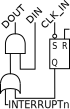
\includegraphics[width=.13\linewidth]{img/glitch_inducer}}
}
%
  \caption{
    Induced Glitch. A node inducing a glitch uses the edge at time~3 to
    de-assert its bus request, instead electing to forward again. At time~4,
    the control node detects no winner of arbitration. The control node
    finishes the arbitration cycle as required by~\label{spec:spurious}. The
    control node then immedaitely Interrupts the bus, indicating failure. An
    inducing node can harvest these clock edges to wake itself. The first set
    of power edges are used to wake the {\tt Bus~Controller}, the second set
    are used by the {\tt Bus~Controller} to wake the entire node.
    Figure~\ref{fig:induced-inducer} shows a simple glitch inducer circuit.
    The {\tt INTERRUPT\_N} line is active low.
  }
  \label{fig:induced}
} % End \figTimingInducedGlitch

